\documentclass{beamer}

% --- THEME AND APPEARANCE ---
\usetheme{Madrid}
\usecolortheme{default}
\setbeamertemplate{navigation symbols}{}
\setbeamertemplate{footline}[frame number]

% --- REQUIRED PACKAGES ---
\usepackage{fontspec}

% --- FIX: SIMPLIFIED BABEL SETUP ---
% We removed 'bidi' and 'provide=*' to stop the \englishdate error
\usepackage[english]{babel}
\babelfont{rm}{Arial}

\usepackage{amsmath}
\usepackage{booktabs}
\usepackage{graphicx}
\usepackage{ragged2e}
\usepackage{tikz}
\usepackage{algpseudocode} % Needed for algorithmic environment

% --- PRESENTATION METADATA ---
\title[Intelligent Network Topology Optimization]{Intelligent Network Topology Optimization Using LAM}
\author{Karan Khotare (BT22CSE111) \and Yash (BT22CSE110) \and Aman Raj (BT22CSE115) \and Om Ashok Nalage (BT22CSE117)}
\institute{Department of Computer Science and Engineering}
\date{\today}
\subject{Final Year Project Presentation}

% --- ADD LOGO TO TITLE PAGE ---
\addtobeamertemplate{title page}{%
  \begin{tikzpicture}[remember picture,overlay]
    \node[anchor=north,yshift=-5.5cm,xshift=.05cm] at (current page.north) {
      % Ensure logo.jpg exists in your folder, or this will error
      
\includegraphics[height=2cm]{logo.jpg}
    };
  \end{tikzpicture}%
}

% --- HELPER COMMAND FOR IMAGE PLACEHOLDERS ---
% CRITICAL FIX: The line "\includegraphics...{logo.png}" was here.
% You cannot put an image directly in the preamble. I have removed it.

\newcommand{\placeholder}[2]{%
  \begin{center}
    \framebox{
      \parbox{0.8\textwidth}{\hspace{2cm}
        \vspace{2cm}
        \textbf{#1}\\[5pt]
        \small\textit{#2}
        \vspace{2cm}
      }
    }
  \end{center}
}
\begin{document}

% --- TITLE PAGE ---
\begin{frame}
  \maketitle
  \begin{center}
    \vspace{1cm}
    \large
    \textbf{Under the guidance of} \\
    Dr. Nidhi Lal
  \end{center}
\end{frame}

% --- TABLE OF CONTENTS ---
\begin{frame}
  \frametitle{Outline}
  \tableofcontents
\end{frame}


% --- SECTION: PHASE 2 IMPLEMENTATION ---
\section{Phase 2: AI-Based Router Recommendation}

% Slide 1: Overview of the AI Approach
\begin{frame}
  \frametitle{Phase 2: AI-Driven Router Selection}
  \begin{block}{Objective}
    To transition from static mathematical formulas (CMBA) to a dynamic \textbf{Machine Learning approach} that predicts the optimal router for caching based on real-time network states.
  \end{block}
  
  \begin{itemize}
      \item \textbf{Input:} Real-time network telemetry data.
      \item \textbf{Process:} Data logging via CSV $\rightarrow$ Model Training $\rightarrow$ Prediction.
      \item \textbf{Output:} The specific Router ID ($R_{best}$) that yields the highest probability of a cache hit and lowest latency.
  \end{itemize}
\end{frame}

% Slide 2: Feature Engineering (The Metrics used)
\begin{frame}
  \frametitle{Feature Engineering \& Data Collection}
  To train our model, we simulated network traffic and logged the following key features into a dataset (\texttt{.csv}):

  \begin{enumerate}
      \item \textbf{Cache Occupancy:} The current percentage of storage used in the router. High occupancy may indicate a need for eviction or bypassing.
      \item \textbf{Cache Hit Ratio (CHR):} Historical performance of the router in serving content.
      \item \textbf{Centrality Measure Value (CMV):} The topological importance of the node (derived from Phase 1).
      \item \textbf{Latency:} The time delay observed at the specific router node.
  \end{enumerate}
  
  \vspace{0.5cm}
  \textit{\small These features serve as the independent variables ($X$) for our predictive model.}
\end{frame}

% --- SLIDE: REAL DATA SNAPSHOT (UPDATED) ---
\begin{frame}
  \frametitle{Dataset Snapshot (Real Telemetry Data)}
  \begin{block}{Live Simulation Logs}
    Below is a sample of the actual telemetry data collected during the evaluation phase. 
    The model analyzes the \textbf{network metrics} to predict the \textbf{Best Router} ($R_{best}$) for the next hop.
  \end{block}

  \begin{table}
    \centering
    \footnotesize
    \renewcommand{\arraystretch}{1.3}
    % Adjusted columns: Req ID, Occupancy, CHR, Prediction
    \begin{tabular}{c c c c}
      \toprule
      \textbf{Req ID} & \textbf{Occupancy} & \textbf{CHR} & \textbf{Predicted $R_{best}$} \\
      \midrule
      % Data from best_router.csv (columns 1, 3, 5, 4)
      0 & 0.724 & 0.598 & \textbf{R19} \\
      1 & 0.825 & 0.587 & \textbf{R19} \\
      2 & 0.804 & 0.572 & \textbf{R19} \\
      3 & 0.786 & 0.558 & \textbf{R19} \\
      4 & 0.777 & 0.539 & \textbf{R12} \\
      \bottomrule
    \end{tabular}
    \caption{Fragment of \texttt{best\_router.csv} showing key metrics and AI predictions.}
  \end{table}
  
  \vspace{0.2cm}
  \textit{\small Note: Occupancy and CHR are normalized values (0-1) used as input features.}
\end{frame}

% Slide 3: The AI Model Details
\begin{frame}
  \frametitle{Model Architecture: Random Forest Classifier}
  We selected an ensemble learning method to handle the non-linear relationships between network metrics.
  
  \begin{alertblock}{Algorithm Selected: Random Forest Classifier}
    \begin{itemize}
        \item \textbf{Why Random Forest?} It is robust against overfitting and handles high-dimensional data effectively by averaging multiple decision trees.
    \end{itemize}
  \end{alertblock}

  \begin{block}{Hyperparameters Configured}
    \begin{itemize}
        \item \textbf{n\_estimators = 200}: We utilized 200 decision trees to ensure stability and reduce variance in predictions.
        \item \textbf{random\_state = 42}: Fixed seed to ensure reproducibility of our evaluation results.
        \item \textbf{Target Variable}: The optimal Router ID for the specific content request.
    \end{itemize}
  \end{block}
\end{frame}

% Slide 4: The Workflow (Summary)
\begin{frame}
  \frametitle{System Workflow}
  \begin{enumerate}
      \item \textbf{Simulation Phase:} The network simulator runs, calculating CMV, Latency, and Occupancy for every transaction.
      \item \textbf{Data Logging:} All feature snapshots are appended to a training CSV file.
      \item \textbf{Training:} The \texttt{RandomForestClassifier(n\_estimators=200)} is trained on this historical data.
      \item \textbf{Inference:} For new packets, the model analyzes current metrics and predicts the "Best Router."
      \item \textbf{Action:} The packet is forwarded or cached at the predicted router, resulting in the performance improvements shown in the following graphs.
  \end{enumerate}
\end{frame}







\begin{frame}
  \frametitle{Performance Graph: Cache Hit Ratio (CHR)}
  \justify
  This graph shows the improvement in Cache Hit Ratio over simulation iterations.
  
  % --- IMAGE PLACEHOLDER ---
  % To add your image, replace the line below with:
 %  \includegraphics[width=0.8\textwidth]{comparison_iter_chr_improved.png}
  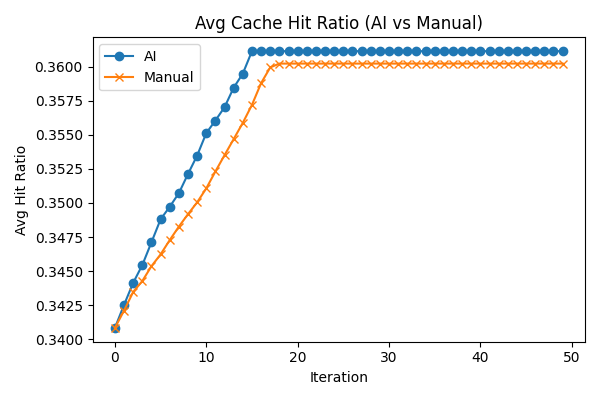
\includegraphics[width=0.8\textwidth]{ai_vs_manual_cache_hit_ratio.png}
\end{frame}

\begin{frame}
  \frametitle{Performance Graph: Cache Occupancy}
  \justify
  This graph illustrates the increase in the percentage of cache occupancy.
  
  % --- IMAGE PLACEHOLDER ---
  % To add your image, replace the line below with:
  % \includegraphics[width=0.8\textwidth]{comparison_iter_hrr_improved.png}
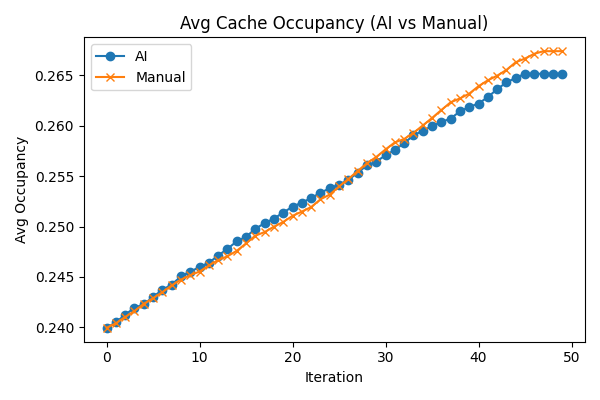
\includegraphics[width=0.8\textwidth]{ai_vs_manual_cache_occupancy.png}
\end{frame}

\begin{frame}
  \frametitle{Performance Graph: Latency}
  \justify
  This graph shows the average latency over number of iterations for AI recommended and Manual Method.

  % --- IMAGE PLACEHOLDER ---
  % To add your image, replace the line below with:
  % \includegraphics[width=0.8\textwidth]{comparison_iter_latency_improved.png}
 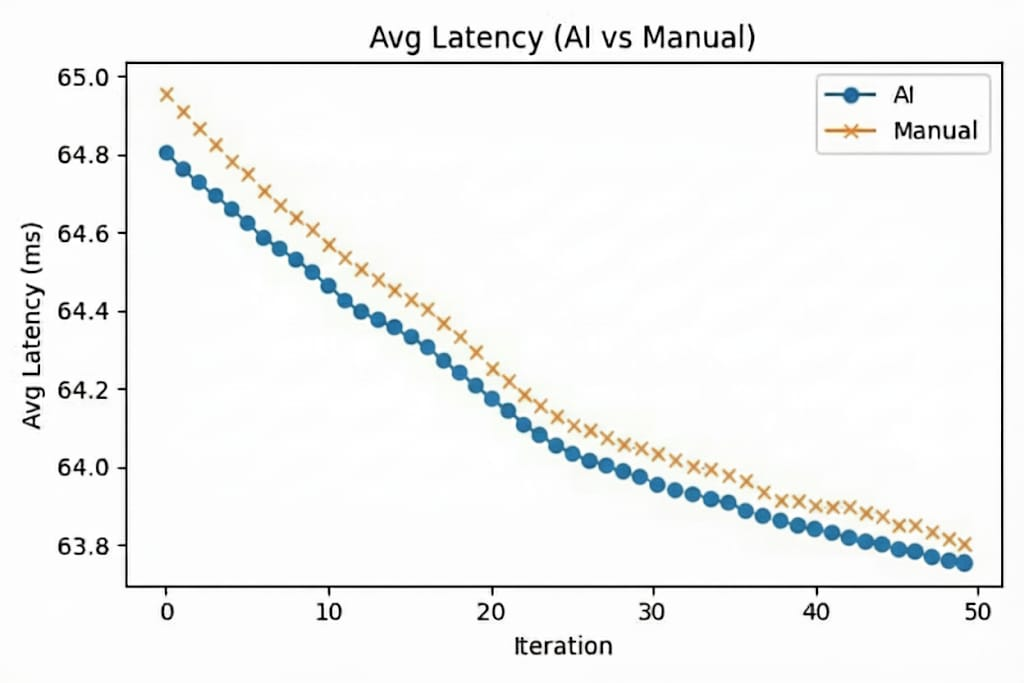
\includegraphics[width=0.8\textwidth]{latency.jpg}

\end{frame}

% --- SECTION: EXPECTED OUTCOMES ---
\section{Expected Outcomes}
\begin{frame}
  \frametitle{Expected Outcomes}
  \begin{itemize}
    \item A more intelligent and adaptive network topology.
    \item Optimized cache placement for better resource utilization.
    \item Reduced content retrieval latency and redundancy in large-scale networks.
  \end{itemize}
\end{frame}

% --- SECTION: TOOLS & TECHNOLOGIES ---
\section{Tools \& Technologies}
\begin{frame}
  \frametitle{Tools \& Technologies}
    \begin{itemize}
        \item \textbf{Simulator:} Custom Python Simulator
        \item \textbf{Algorithms:} Centrality Measures (CMBA), Reinforcement Learning (Q-Learning / Deep RL)
        \item \textbf{Languages:} Python
        \item \textbf{Evaluation Metrics:} Cache hit ratio, server hit reduction, hop reduction, latency, and throughput.
    \end{itemize}
\end{frame}

% --- SECTION: CONCLUSION ---
\section{Conclusion}
\begin{frame}
  \frametitle{Conclusion}
  Our project aims to:
  \begin{itemize}
    \item Develop a scalable and intelligent topology optimization framework.
    \item Extend the centrality-based selection mechanism using a Large Action Model (LAM).
    \item Ultimately, create a more efficient Content-Centric Network for modern data demands.
  \end{itemize}
\end{frame}

% --- SECTION: FUTURE WORKS TO BE DONE ---
\section{Next Phase}
\begin{frame}
  \frametitle{Next Phase}
  \begin{block}{Core Idea}
    To develop a Deep Reinforcement Learning (DRL) agent that dynamically optimizes caching and routing decisions in the network.
  \end{block}
  \begin{block}{Objectives}
    \begin{itemize}
        \item Implement and evaluate the baseline CMBA.
        \item Integrate a DRL agent to enhance decision-making.
        \item Evaluate overall performance improvement in terms of:
        \begin{itemize}
            \item Cache Hit Ratio (CHR)
            \item Hop Reduction Ratio (HRR)
            \item Latency \& Throughput
        \end{itemize}
    \end{itemize}
  \end{block}
\end{frame}

% --- SECTION: REFERENCES ---
\section{References}
\begin{frame}
  \frametitle{References}
  \begin{thebibliography}{99}
    \bibitem{lal2017}
    Kumari Nidhi Lal, Anoj Kumar (2017).
    \newblock A Centrality-measures based Caching Scheme for Content-centric Networking (CCN).
    \newblock \textit{Multimedia Tools and Applications}.
    
    \bibitem{fyp2024}
    AI-Driven Dynamic Cache Policy Selection in Information-Centric Networking (FYP Thesis 2024-25).

  \end{thebibliography}
\end{frame}

% --- FINAL SLIDE ---
\begin{frame}
  \centering
  \vspace*{2cm}
  \Huge\bfseries Thank You
  \vfill
  \Large Questions?
\end{frame}

\end{document}
% =================================================================
% --- END PRESENTATION ---
% =================================================================